This chapter concerns itself with the problem at the heart of this thesis: the
TMOR problem introduced in Section~\ref{sec:mot_symmetry_reduction}. In
Section~\ref{sec:tmor_definition} we will first formalize the TMOR problem in
light of the theoretical foundations laid out in Chapter~\ref{chap:theo} and
then describe some algorithms that address it in
Section~\ref{sec:tmor_algorithmic_approaches}. Finally,
Section~\ref{sec:tmor_optimization_via_decomposition} will introduce some
important optimizations for certain types of separable and hierarchical
architecture graphs. We will not consider partial symmetries in this chapter,
for one because most of what is discussed here\footnote{Except optimization by
decomposition.}applies to them equally and for another because, as we have seen
previously, the algorithms we use for determining and representing them are not
quite efficient enough to be useful in practice.

\section{Definition}
\label{sec:tmor_definition}

In Chapter~\ref{chap:ag} we have seen how to model abstract MPSoC architectures
as undirected graphs and how to describe their symmetries and partial
symmetries by finding the automorphism groups and partial automorphism inverse
monoids of these undirected graphs respectively. In a similar manner we will now
formalize what we mean when we say ``task mapping'' and relate this concept
to that of architecture graphs.

\begin{defn}{Task Mapping}
  Given an architecture graph $A = (P, C, \mathrm{col}_P,
  \mathrm{col}_C)$, a $k$-task mapping is a sequence $T_A^k = (t_1, t_2,
  \dots, t_k), t_i \in P, \forall 1 \leq i \leq k$. Instead of $t_i$ we also
  write $T_{A}^k[i]$.
\end{defn}

\begin{exmp}[label=exmp:task_mapping]{Task Mapping}
  Consider again the task mappings presented in
  Figure~\ref{fig:regular_mesh_4_4_mappings}, and assume that for the given
  abstract MPSoC architecture we construct the architecture graph
  presented in Figure~\ref{fig:architecture_graph_4_4}. Then the task mappings
  (a)-(d) are described by:
  %
  \begin{itemize}
    \item (a) $\rightarrow (1, 5, 9, 13)$
    \item (b) $\rightarrow (1, 9, 5, 13)$
    \item (c) $\rightarrow (1, 2, 3, 4)$
    \item (d) $\rightarrow (2, 6, 10, 14)$
  \end{itemize}
  %
  \begin{figure}[H]
    \centering
    \begin{tikzpicture}
      % vertices
      \Vertex[x=0,y=0,L=$1$]{1}
      \Vertex[x=1.5,y=0,L=$2$]{2}
      \Vertex[x=3,y=0,L=$3$]{3}
      \Vertex[x=4.5,y=0,L=$4$]{4}
      \Vertex[x=0,y=-1.5,L=$5$]{5}
      \Vertex[x=1.5,y=-1.5,L=$6$]{6}
      \Vertex[x=3,y=-1.5,L=$7$]{7}
      \Vertex[x=4.5,y=-1.5,L=$8$]{8}
      \Vertex[x=0,y=-3,L=$9$]{9}
      \Vertex[x=1.5,y=-3,L=$10$]{10}
      \Vertex[x=3,y=-3,L=$11$]{11}
      \Vertex[x=4.5,y=-3,L=$12$]{12}
      \Vertex[x=0,y=-4.5,L=$13$]{13}
      \Vertex[x=1.5,y=-4.5,L=$14$]{14}
      \Vertex[x=3,y=-4.5,L=$15$]{15}
      \Vertex[x=4.5,y=-4.5,L=$16$]{16}
      % horizontal edges
      \Edge(1)(2)
      \Edge(2)(3)
      \Edge(3)(4)
      \Edge(5)(6)
      \Edge(6)(7)
      \Edge(7)(8)
      \Edge(9)(10)
      \Edge(10)(11)
      \Edge(11)(12)
      \Edge(13)(14)
      \Edge(14)(15)
      \Edge(15)(16)
      % vertical edges
      \Edge(1)(5)
      \Edge(2)(6)
      \Edge(3)(7)
      \Edge(4)(8)
      \Edge(5)(9)
      \Edge(6)(10)
      \Edge(7)(11)
      \Edge(8)(12)
      \Edge(9)(13)
      \Edge(10)(14)
      \Edge(11)(15)
      \Edge(12)(16)
    \end{tikzpicture}
    \caption{Architecture graph corresponding to abstract MPSoC architecture
             presented in Figure~\ref{fig:regular_mesh_4_4_mappings}.}
    \label{fig:architecture_graph_4_4}
  \end{figure}
\end{exmp}
%
In general, we will not always be interested in \textit{every} possible task
mapping for a given architecture graph. For example, we might not be interested
in task mappings which map two or more tasks to the same processing element.
To formalize this notion, we introduce the concept of \textit{task mapping spaces}:

\begin{defn}{Task Mapping Space}
  Given an architecture graph $A = (P,C, \operatorname{col}_P,
  \operatorname{col}_C)$, we denote the space of all admissible $k$-task mappings
  on $A$ by $\Theta_A^k$ and note that $\Theta_A^k \subseteq P^k$.
\end{defn}

\begin{exmp}[label=exmp:task_mapping_space]{Task Mapping Space}
  The $k$-task mapping space for the architecture graph from
  Example~\ref{exmp:task_mapping} which only admits task mappings for which no
  two tasks share the same processing element is $\Theta_A^k \subset
  \{1,2,\dots,16\}^k$ such that $\forall T_A^k \in \Theta_A^k: i \neq j \implies
  T_{A}^k[i] \neq T_{A}^k[j]$.
\end{exmp}
%
Remember that we are interested in finding task mappings that are equivalent by
symmetry. We can find such task mappings via the automorphisms of $A$
represented as permutations as follows:

\begin{defn}{Task Mapping Permutation}
  Given an architecture graph $A = (P,C, \operatorname{col}_P,
  \operatorname{col}_C)$, a $k$-task mapping $T_A^k = (t_1, t_2, \dots, t_k) \in
  \Theta_A^k$ and a permutation $g$ over $P$, we define $g: \Theta_A^k \to
  \Theta_A^k$ with:
  %
  \begin{equation*}
     g(T_A^k) = \begin{cases}
                   (g(t_1), g(t_2), \dots, g(t_k)),
                     &\text{if}\ (g(t_1), g(t_2), \dots, g(t_k)) \in \Theta_A^k \\
                   \text{undefined},
                     &\text{otherwise}
                 \end{cases}
  \end{equation*}
  %
  From now on we assume that if $G$ is the automorphism group of $A$, then
  $\forall T_A^k \in \Theta_A^k: \forall g \in G: g(T_A^k) \in \Theta_A^k$
  (alternatively: we assume that $\Theta_A^k$ is a $G$-set) such that the
  following discussions about task mapping orbits make sense.
\end{defn}

\begin{exmp}{Task Mapping Permutation}
  As we shall see in Example~\ref{exmp:task_mapping_orbit}, the permutation $g
  = (1\ 4)(2\ 3) (5\ 8)(6\ 7)(9\ 12)(10\ 11)(13\ 16)(14\ 15)$ is an automorphism
  of the architecture graph from Example~\ref{exmp:task_mapping} and it holds
  e.g. that $g((1,5,9,13)) = (4,8,12,16)$.
\end{exmp}
%
If we seek to determine \textit{all} task mappings equivalent by symmetry to a
given task mapping we can again make use of the concept of group orbits
introduced in Definition~\ref{defn:group_orbit}. By introducing a strict
ordering on any task mapping space we can furthermore find a canonical
representative for any such orbit, analogous to Definition~\ref{defn:sim}. This
is everything we need to formalize the TMOR problem: In theory, given an
architecture graphs automorphism group, we can partition any task mapping space
into orbits and then reduce these orbits to their canonical representatives.

\begin{defn}[label=defn:task_mapping_ordering]{Task Mapping Ordering}
  On any $k$-task mapping space $\Theta_A^k$ we define a total strict ordering
  $\operatorname{<} \subseteq \Theta_A^k \times \Theta_A^k$ as follows:
  %
  Let $T_A^k = (t_1, t_2, \dots, t_k), \widetilde{T}_A^k = (\widetilde{t}_1,
  \widetilde{t}_1, \dots, \widetilde{t}_k) \in \Theta_A^k$ then:
  %
  \begin{equation*}
    (T_A^k, \widetilde{T}_A^k) \in \operatorname{<}
      \Leftrightarrow
    \exists 1 \leq i \leq k:
      (\forall 1 \leq j < i: t_j = \widetilde{t}_j) \land (t_i < \widetilde{t}_i)
  \end{equation*}
  %
  This type of ordering is called \textit{lexicographical}. We also write
  $T_A^k < \widetilde{T}_A^k$.
\end{defn}

\begin{exmp}{Task Mapping Ordering}
  For the task mappings from Example~\ref{exmp:task_mapping} it holds that:
  %
  \begin{equation*}
    (1,2,3,4) < (1,5,9,13) < (1,9,5,13) < (2,6,10,14)
  \end{equation*}
\end{exmp}

\begin{defn}[label=exmp:task_mapping_orbit]{Task Mapping Orbit}
  Given a permutation group $G$ and a task mapping space $\Theta_A^k$, we
  define the orbit of some task mapping $T_A^k \in \Theta_A^k$ as $T_A^{k,G} =
  [T_A^k]_{\sim_G} = \{g(T_A^k) \mid g \in G\}$. We also define
  $\operatorname{repr}(T_A^{k,G})$ analogous to Definition~\ref{defn:sim}, with
  $<$ as in Definition~\ref{defn:task_mapping_ordering}. When $G$ is the
  automorphism group of $A$ we simply write $\operatorname{repr}(T_A^k)$.
\end{defn}

\begin{exmp}{Task Mapping Orbits}
  Consider again the architecture graph $A$ from
  Example~\ref{exmp:task_mapping} and the task mapping space $\Theta_A^k$ from
  Example~\ref{exmp:task_mapping_space}.
  %
  We can now formally determine which task mappings are equivalent by symmetry
  to e.g.  $T_{A,1}^4 = (1, 5, 9, 13)$. This is analogous to determining
  $T_{A,1}^{4,G}$ where $G$ is the automorphism group of $A$.
  %
  It is well known that the automorphism group $G$ of any $n \times n$ regular
  mesh architecture graph $A$ is ismorphic to the \textit{dihedral group} $D_8$
  with $|D_8| = 8$. It holds that:
  %
  \begin{align*}
    G = \langle\{&(1\ 4)(2\ 3)(5\ 8)(6\ 7)(9\ 12)(10\ 11)(13\ 16)(14\ 15), \\
                 &(2\ 5)(3\ 9)(4\ 13)(7\ 10)(8\ 14)(12\ 15)\}\rangle
  \end{align*}
  %
  which we can interpret geometrically as reflections about the meshes upper
  left to lower right diagonal and its vertical center respectively. As can be
  readily verified, we have:
  %
  \begin{align*}
    T_{A,1}^{k,G} = \{
      &(1, 2, 3, 4),
      (1, 5, 9, 13),
      (4, 3, 2, 1),
      (4, 8, 12, 16),\\
      &(13, 14, 15, 16),
      (13, 9, 5, 1),
      (16, 12, 8, 4),
      (16, 15, 14, 13)
    \}
  \end{align*}
  %
  And $\operatorname{repr}(T_{A,1}^k) = (1, 2, 3, 4)$.
  %
  We can determine how many task mapping orbits there are in total by making use of
  Lemma~\ref{lemma:cauchy_frobenius}: For all $g \in G$, let $\Theta_A^{k, g} =
  \{T_A^k \in \Theta_A^k \mid g(T_A^k) = T_A^k\}$ and note that:
  %
  \begin{equation*}
    |\Theta_A^{k,g}| = \begin{cases}
                         \frac{|P^g|!}{(|P^g| - k)!}, &\text{if}\ |P^g| \geq k\\
                         0,                           &\text{otherwise}
                       \end{cases}
  \end{equation*}
  %
  as should be obvious from the definition of $\Theta_A^k$. We have:
  %
  \begin{equation*}
    \begin{split}
      &|\Theta_A^{k,()}| = \nicefrac{16!}{12!} = 43680 \\
      &|\Theta_A^{k,(1\ 13)(2\ 14)(3\ 15)(4\ 16)(5\ 9)(6\ 10)(7\ 11)(8\ 12)}| = 0 \\
      &|\Theta_A^{k,(1\ 13\ 16\ 4)(2\ 9\ 15\ 8)(3\ 5\ 14\ 12)(6\ 10\ 11\ 7)}| = 0 \\
      &|\Theta_A^{k,(1\ 16)(2\ 12)(3\ 8)(5\ 15)(6\ 11)(9\ 14)}| = \nicefrac{4!}{0!} = 24 \\
      &|\Theta_A^{k,(1\ 16)(2\ 15)(3\ 14)(4\ 13)(5\ 12)(6\ 11)(7\ 10)(8\ 9)}| = 0 \\
      &|\Theta_A^{k,(1\ 4)(2\ 3)(5\ 8)(6\ 7)(9\ 12)(10\ 11)(13\ 16)(14\ 15)}| = 0 \\
      &|\Theta_A^{k,(1\ 4\ 16\ 13)(2\ 8\ 15\ 9)(3\ 12\ 14\ 5)(6\ 7\ 11\ 10)}| = 0 \\
      &|\Theta_A^{k,(2\ 5)(3\ 9)(4\ 13)(7\ 10)(8\ 14)(12\ 15)}| = \nicefrac{4!}{0!} = 24 \\
    \end{split}
  \end{equation*}
  %
  By averaging these set sizes we obtain $\frac{1}{8}(43680 + 24 + 24) = 5466$.
  Since $|\Theta_A^k| = \frac{16!}{14!} = 43680$, if we could successfully
  determine representatives for every orbit of $G$, we would effectively reduce
  the size of the task mapping search space by a factor of $\frac{43680}{5466}
  \approx 8$.
\end{exmp}

\section{Algorithmic Approaches}
\label{sec:tmor_algorithmic_approaches}

\begin{algorithm}
  \caption{Obtain orbit identifier.}
  \label{alg:tmor}
  \begin{algorithmic}[1]
  \Procedure{ORBIT\_IDENTIFIER}{$T_A^k$}
    \LineComment{$\mathrm{reprs}$ retains its state across invocations.}
    \\
    \If{$A$ has changed since last invocation}
       \State $\mathrm{reprs} \gets ()$
    \EndIf
    \\
    \If{$\operatorname{repr}(T_A^k) \notin \mathrm{reprs}$}
      \State Append $\operatorname{repr}(T_A^k)$ to $\mathrm{reprs}$
    \EndIf
    \\
    \State \textbf{return} index of $\operatorname{repr}(T_A^k)$ in $\mathrm{reprs}$
  \EndProcedure
  \end{algorithmic}
\end{algorithm}

It now remains to discuss how we can partition a task mapping space in
practice. Because $|\Theta_A^k|$ might be very large, in general it is
impractical to explicitly determine all orbits for a given automorphism group.
An iterative approach is more feasible: We consider a series of task mappings
in turn and for each of them determine the canonical representative of the
orbit it lies in. In this way, for every new task mapping we can discern
whether we have already encountered a task mapping in the same orbit earlier
(and can thus e.g. skip some expensive simulation step for this new task
mapping) by matching canonical representatives.  Algorithm~\ref{alg:tmor} is a
formalization of this. It takes as its argument a task mapping and returns an
integer uniquely identifying the orbit in which this task mapping lies. The
central importance of orbit representatives to this approach is why introduced
the term TMOR.

Algorithm~\ref{alg:tmor} is particularly interesting because it lends itself to
be used in conjunction with e.g. a genetic algorithm which generates new
``interesting'' task mappings based on the simulated characteristics of old
ones. We can then simply discard those task mappings that are equivalent by
symmetry to, i.e. lie in the same orbit as, previously generated ones.

\begin{algorithm}
  \caption{Determine canonical representatives via orbit enumeration.}
  \label{alg:task_repr_orbit}
  \begin{algorithmic}[1]
  \Procedure{TMOR\_ORBIT}{$T_A^k$, $G = \left<S\right>$}
    \LineComment{$G$ is the automorphism group of $A$.}
    \\
    \State $\mathrm{orbit} \gets \{\}$

    \While{$\mathrm{orbit}$ is changing}
      \For{$\widetilde{T}_A^k \in \mathrm{orbit}$, $g$ in $S$}
        \State $\mathrm{orbit} \gets
                 \mathrm{orbit} \cup \{g(\widetilde{T}_A^k)\}$
      \EndFor
    \EndWhile
    \\
    \State \textbf{return} $\min(\mathrm{orbit})$
  \EndProcedure
  \end{algorithmic}
\end{algorithm}

\begin{algorithm}
  \caption{Determine canonical representatives via group enumeration.}
  \label{alg:task_repr_iterate}
  \begin{algorithmic}[1]
  \Procedure{TMOR\_ITERATE}{$T_A^k$, $G$}
    \LineComment{$G$ is the automorphism group of $A$.}
    \\
    \State $\operatorname{repr}(T_A^k) \gets T_A^k$

    \For{$g \in G$}
      \If{$g(T_A^k) < \operatorname{repr}(T_A^k)$}
        \State $\operatorname{repr}(T_A^k) \gets g(T_A^k)$
      \EndIf
    \EndFor
    \\
    \State \textbf{return} $\operatorname{repr}(T_A^k)$
  \EndProcedure
  \end{algorithmic}
\end{algorithm}

\begin{algorithm}
  \caption{Determine canonical representatives via local search.}
  \label{alg:task_repr_local_search}
  \begin{algorithmic}[1]
  \Procedure{TMOR\_LOCAL\_SEARCH}{$T_A^k$, $G = \left<S\right>$}
    \LineComment{$G$ is the automorphism group of $A$.}
    \\
    \State $\operatorname{repr}(T_A^k) \gets T_K^k$
    \While{$\operatorname{repr}(T_A^k)$ is changing}
      \State $\operatorname{repr}(T_A^k) \gets
               \min(\{g(\operatorname{repr}(T_A^k)) \mid g \in S\})$
    \EndWhile
    \\
    \State \textbf{return} $\operatorname{repr}(T_A^k)$
  \EndProcedure
  \end{algorithmic}
\end{algorithm}

In order to implement Algorithm~\ref{alg:tmor}, we need to be
able to efficiently determine $\operatorname{repr}(T_A^k)$. If we desire
guaranteed correctness there are two basic approaches which both completely
enumerate $T_A^{k,G}$: We either enumerate the orbit explicitly via the fixed
point Algorithm~\ref{alg:task_repr_orbit} or by iterating over the elements of
$G$ as in Algorithm~\ref{alg:task_repr_iterate}. We will also refer to these
algorithms as \textit{bruteforce orbit enumeration} and \textit{bruteforce
iteration} respectively.

If we (as is usually the case) want to find canonical representatives for a
large number of task mappings, we can potentially improve performance in both
cases by hashing already discovered canonical representatives and aborting the
task mapping orbit discovery when a known canonical representative is
encountered. We could also choose to additionally hash a number of random task
mappings per orbit in an attempt to abort the enumeration earlier.

It is hard to say in general if bruteforce orbit enumeration or iteration is
more efficient for a given automorphism group.  Overall, bruteforce iteration
seems to be most suitable if $|G|$ is small and bruteforce orbit enumeration if
$\Theta_A^k$ is partitioned into many small orbits by $G$. Unfortunately, this
latter characteristic is not easily determinable without actually computing the
complete orbit partition.  We shall analyse this matter more thorougly in
Section~\ref{sec:tmor_complexity_and_accuracy_considerations}.

If both methods of orbit enumeration prove to be impractically slow, we can
employ Algorithm~\ref{alg:task_repr_local_search} which computes an
\textit{approximate} canonical representative via local search. In effect, this
algorithm performs breadth first search within an orbit. The returned canonical
representative is thus not guaranteed to be the correct one which might be
acceptable depending on the application and likelihood that this will occur.
Note that it might be sensible to append additional elements to the generating
set $S$, e.g. $\{g^{-1} \mid g \in S\}$ or random elements of $G$, in order to
``widen'' the search tree and/or to employ e.g. simulated annealing or similar
heuristic techniques instead of breadth first search, refer to
e.g.\cite{Russell}. These potential improvements are however beyond the scope
of this thesis.

\section{Complexity and Accuracy Considerations}
\label{sec:tmor_complexity_and_accuracy_considerations}

The time complexity of bruteforce iteration is clearly $O(|G|)$.  Furthermore,
the execution time of bruteforce iteration should not vary substantially with
$k$, assuming that iterating through $G$ is more computationally expensive than
finding $g(T_{A}^k)$.

At worst, bruteforce orbit iteration only adds a single element to $T_A^{k,G}$
in every iteration and its runtime complexity is thus $O(|S| (1 + 2
+ \dots + (|T_A^{k,G}| - 1))) = O(|S| |T_A^{k,G}|^2)$. If
$\Theta_{A}^k$ is partitioned into relatively few but large orbits, finding
representatives via orbit enumeration is potentially prohibitively expensive.

As we have demonstrated in Example~\ref{exmp:cauchy_frobenius}, determining the
number of task mapping orbits for a given automorphism group $G$ is possible
algorithmically in $O(|G|)$ time by making use of
Lemma~\ref{lemma:cauchy_frobenius}. Since these orbits partition
$\Theta_{A}^k$, we also know that their sizes must sum to $|\Theta_{A}^k|$ and
we can thus easily determine the \textit{average} orbit size. However, the
total execution time of the bruteforce orbit enumeration algorithm largely
depends on the size of the \textit{largest} orbit or orbits\footnote{This does
not hold if $G$ partitions $\Theta_A^k$ into a large number of very small
orbits and relatively few large ones whose combined size is still small
compared to $|\Theta_A^k|$. We shall not analyse when or if this occurs in
detail.}. There are two reasons for this:

\begin{itemize}
\item For a given task mapping $T_{A}^k$ the runtime complexity of the
bruteforce orbit enumeration algorithm grows superlinearly with
$|T_{A}^{k,G}|$ as described above.

\item For two orbits, one significantly larger than the other, the probability
of some $T_A^k$ randomly drawn from a uniform distribution over $\Theta_A^k$
lying in the larger orbit is greater than the probability of it lying in the
smaller orbit.
\end{itemize}

\noindent
Unfortunately, it is very difficult to determine a tight upper bound for the
size of any given orbit for even moderately large values of $k$. We can however
trivially state that any orbit can at most be of size $|G|$, irrespective of
$|\Theta_A^k|$. This is because every element in an orbit is ``reachable'' from
every other element in the same orbit via some $g \in G$, i.e. $\forall T_A^k
\in \Theta_A^k: \forall T_{A,1}^k, T_{A,2}^k \in T_A^{k,G}: \exists g \in G:
g(T_{A,1}^k) = T_{A,2}^k$\footnote{It can additionally be shown that the size
of every orbit must \textit{divide} $|G|$. In theory we could use this fact to
find one or several possibilities for the orbit size distribution by looking
for an integer partition of $|\Theta_A^k|$ which has
$|\bigslant{\Theta_A^k}{\sim_G}|$ summands $\in \{s \in \mathbb{N}_+ \mid s
\mid |G|\}$.  However, because the number of orbits is typically very large
even for moderately large values of $k$, known integer partition algorithms
cannot cope with this task, refer to e.g.~\cite{Zoghbi}.}. This also implies that
$O(\left<S\right> |T_A^{k,G}|^2) = O(\left<S\right> |G|^2)$.

It remains to ask whether we expect the average orbit size to increase with
$k$. A simple observation shows that this is almost certainly the case:
Assuming again that no two tasks can be mapped to the same processing element
it trivially holds that $|\Theta_A^{k+1}| = (|P| - k) \cdot |\Theta_A^k|$.
Thinking back to Example~\ref{exmp:cauchy_frobenius}, for the number of orbits
of $\Theta_A^k$ we have:
%
\begin{equation*}
 |\bigslant{\Theta_A^k}{\sim_G}| =
 \frac{1}{|G|} \sum_{g \in G} |\Theta_A^{k,g}|
\end{equation*}
%
with:
%
\begin{equation*}
 |\Theta_A^{k,g}| =
 \begin{cases}
   \frac{|P^g|!}{(|P^g| - k)!}, &\text{if}\ |P^g| \geq k\\
   0,                           &\text{otherwise}
 \end{cases}
\end{equation*}
%
Since $\forall g \in G: |P^g| \leq |P|$ we thus have
$|\Theta_A^{k+1,g}| \leq (|P| - k) \cdot |\Theta_{A}^{k,g}|$. And thus
for the average orbit size it holds that:
%
\begin{equation*}
  \frac{|\Theta_A^{k+1}|}{|\bigslant{\Theta_A^{k+1}}{\sim_G}|}
    \geq
  \frac{|\Theta_A^k|}{|\bigslant{\Theta_A^k}{\sim_G}|}
\end{equation*}
%
i.e. the average orbit size cannot decrease with $k$. Thus we can reasonably
expect bruteforce orbit enumeration to perform worse for larger
values of $k$.

The runtime complexity of the local search algorithm obviously mainly depends
on the size of the chosen generating set for $G$. On the other hand, a larger
generating set may sometimes make finding correct representatives more likely,
i.e. it can potentially be sensible to trade off execution time for increased
accuracy by adding redundant elements to $G$'s generating set during local
search as described previously.

In general, we expect local search to execute faster than bruteforce iteration
or orbit enumeration, especially for large values of $|G|$ such that our main
concern with this algorithm is accuracy. A trivial observation we can make here
is that, as with the execution time of bruteforce orbit enumeration, this
metric should mainly depend on the orbit size distribution. This is because
during local search we never ``leave'' a task mapping's orbit, such that smaller
orbits make it more likely that the representative returned is the correct one.
Note that there may be pathological cases where local search never or almost
never produces correct representatives for a given automorphism group and
generating set but investigating whether and when this happens is beyond the
scope of this thesis.

In conclusion, the performance of bruteforce iteration and orbit enumeration as
well as local search depends directly or indirectly (via an upper bound on the
orbit size) on $|G|$. Only bruteforce enumeration is likely to be significantly
impacted by $k$.

\section{Optimization via Decomposition}
\label{sec:tmor_optimization_via_decomposition}

As we discussed in Section\ref{sec:ag_automorphism_decomposition}, we can
decompose the automorphism groups of certain separable and hierarchical
architecture graphs into direct and wreath products. We can make use of this to
potentially decrease the execution time of the algorithms presented in the
previous section. This idea was first presented in~\cite{Donaldson} in the
context of model checking, see also~\cite{DonaldsonThesis}.

Essentially, decomposition allows us to solve the task mapping problem
separately for smaller permutation groups than the full automorphism group.
Algorithms~\ref{alg:task_repr_direct_prod} and~\ref{alg:task_repr_wreath_prod}
demonstrate how this works for the case of direct and wreath product
decomposition respectively. For a definition of $\sigma(G_{\mathrm{proto}}) =
\{\sigma_i(G_{\mathrm{proto}}) \mid 1 \leq i \leq
\operatorname{deg}(G_{\mathrm{super}})\}$ and $\sigma(G_{\mathrm{super}})$ and
proof of correctness of these algorithms refer to~\cite{Donaldson}. Note that
it is possible to employ these algorithms recursively, i.e. we could decompose
an automorphism group into a direct or wreath product and further decompose the
components of this product into direct or wreath products themselves.

\begin{algorithm}
  \caption{Determine canonical representatives for separable architecture graphs.}
  \label{alg:task_repr_direct_prod}
  \begin{algorithmic}[1]
  \Procedure{TMOR\_DIRECT\_PROD}{$T_A^k$, $G_1, \dots, G_n$}
    \LineComment{$G_1 \times \dots \times G_n$ is the automorphism group of $A$.}
    \LineComment{$\operatorname{TMOR}$ is any canonical
                 representative algorithm.}
    \\
    \State $\operatorname{repr}(T_A^k) \gets
           \operatorname{TMOR}(T_A^k, G_1)$
    \\
    \For{$i = 2 \dots n$}
      \State $\operatorname{repr}(T_A^k) \gets
             \operatorname{TMOR}(\operatorname{repr}(T_A^k), G_i)$
    \EndFor
    \\
    \State \textbf{return} $\operatorname{repr}(T_A^k)$
  \EndProcedure
  \end{algorithmic}
\end{algorithm}

\begin{algorithm}
  \caption{Determine canonical representatives for hierarchical architecture graphs.}
  \label{alg:task_repr_wreath_prod}
  \begin{algorithmic}[1]
  \Procedure{TMOR\_WREATH\_PROD}{%
    $T_A^k$, $G_{\operatorname{proto}}, \dots, G_{\operatorname{super}}$}

    \LineComment{$G_{\operatorname{proto}} \wr G_{\operatorname{super}}$ is the
                 automorphism group of $A$.}
    \LineComment{$|\sigma_i(G_{\mathrm{proto}})| = |G_{\mathrm{proto}}|,
                 \forall 1 \leq i \leq \operatorname{deg}(G_{\mathrm{super}})$
                 and $|\sigma(G_{\mathrm{super}})| = |G_{\mathrm{super}}|$.}
    \LineComment{$\operatorname{TMOR}$ is any canonical
                 representative algorithm.}
    \\
    \State $\operatorname{repr}(T_A^k) \gets T_A^k$
    \\
    \For{$i = 1 \dots \operatorname{deg}(G_{\operatorname{super}})$}
      \State $\operatorname{repr}(T_A^k) \gets
                \operatorname{TMOR}(
                  \operatorname{repr}(T_A^k),
                  \sigma_i(G_{\operatorname{proto}}))$
    \EndFor
    \\
    \State \textbf{return} $\operatorname{TMOR}(
                              \operatorname{repr}(T_A^k),
                              \sigma(G_{\operatorname{super}}))$
  \EndProcedure
  \end{algorithmic}
\end{algorithm}

We can especially expect hierarchical decomposition to result in significant
speedups because the combined order of two permutation groups
$G_{\mathrm{proto}}$ and $G_{\mathrm{super}}$\footnote{And thus of all
$\sigma_i(G_{\mathrm{proto}})$ and $\sigma(G_{\mathrm{super}})$.} making up a
wreath product $G = G_{\mathrm{proto}} \wr G_{\mathrm{super}}$ is usually much
smaller than the order of the wreath product itself.
